\documentclass[conference]{IEEEtran}

\IEEEoverridecommandlockouts

\usepackage{setspace}
\usepackage{enumerate}
\usepackage{cite}
\usepackage{times}
\usepackage{url}
\usepackage{graphicx}
%\usepackage{subfigure}
\usepackage{amsmath}
\usepackage{algorithm}
\usepackage{algpseudocode}
\usepackage{pifont}
\usepackage{graphicx}
\usepackage{color}

\newcommand{\refalg}[1]{Algorithm~\ref{#1}}
\newcommand{\refeqn}[1]{Equation~\ref{#1}}
\newcommand{\reffig}[1]{Figure~\ref{#1}}
\newcommand{\reftbl}[1]{Table~\ref{#1}}
\newcommand{\refsec}[1]{Section~\ref{#1}}
\newcommand{\method}[1]{\mbox{\textsc{#1}}}

%\newcommand{\reminder}[1]{\textcolor{red}{[[  #1 ]]}\typeout{#1}}
\newcommand{\reminder}[1]{}

\newcommand{\system}{ENTICE}
\newcommand{\systemfull}{ENTIty Centric  Expansion}

\newtheorem{theorem}{Theorem}[section]
\newtheorem{claim}[theorem]{Claim}

\usepackage{array}
\newcolumntype{L}[1]{>{\raggedright\let\newline\\\arraybackslash\hspace{0pt}}m{#1}}
\newcolumntype{C}[1]{>{\centering\let\newline\\\arraybackslash\hspace{0pt}}m{#1}}
\newcolumntype{R}[1]{>{\raggedleft\let\newline\\\arraybackslash\hspace{0pt}}m{#1}}

\setlength\extrarowheight{2pt} 

\begin{document}
\title{An Entity-centric Approach for Overcoming \\Knowledge Graph Sparsity}
\author{
\IEEEauthorblockN{
Manjunath Hegde,
Partha Talukdar
}
\IEEEauthorblockA{Department~of~Computational~and~Data~Sciences\\
Indian Institute of Science, Bangalore, India\\
manjunath@ssl.serc.iisc.in,
ppt@cds.iisc.ac.in
}
}
\maketitle

\begin{abstract}

Automatic construction of knowledge graphs (KGs) from unstructured text has received considerable attention in recent research, resulting in the construction of several KGs with 
millions of entities (nodes) and facts (edges) among them. Unfortunately, such KGs tend to be severely sparse in terms of number of facts known for a \emph{given} entity, i.e., have low 
\emph{knowledge density}. For example, the NELL KG consists of only 1.34 facts per entity. Unfortunately, such low knowledge density makes it challenging to use  such KGs in real-world 
applications. In contrast to \emph{best-effort} extraction paradigms followed in the construction of such KGs, in this project we argue in favor of \systemfull{} (\system{}), an \emph{entity-centric}
KG population framework, to alleviate the low knowledge density problem in existing KGs. By using \system{}, we are able to increase NELL's knowledge density 
by a factor of 7.7 at 75.5\% accuracy. Additionally, we are also able to extend the ontology discovering new relations and entities. 
\end{abstract}

\section{Introduction}
\label{sec:intro}

%{\newcommand\T{\rule{0pt}{4ex}}


Over the last few years, automatic construction of knowledge graphs (KGs) from web-scale text data has received considerable attention, resulting in the construction of several large KGs such as NELL \cite{mitchell2015never}, Google's Knowledge Vault \cite{dong2014knowledge}. These KGs consist of millions of entities and facts involving them. While measuring size of the KGs in terms of number of entities and facts is helpful, they don't readily capture the volume of knowledge needed in real-world applications. When such a KG is used in an application, one is often interested in known facts for a \emph{given} entity, and not necessarily the overall size of the KG. In particular, knowing the average number of facts per entity is quite informative. We shall refer to this as the \textit{knowledge density} of the KG. %Please note that a sparse KG will also have low knowledge density.

Low knowledge density (or high sparsity) in automatically constructed KGs has been recognized in recent research \cite{west2014knowledge}. For example, NELL KG has a knowledge density of 1.34. Such low knowledge density puts significant limitations on the utility of these KGs. Construction of such KGs tend to follow a batch paradigm: the knowledge extraction system makes a full pass over the text corpus extracting whatever knowledge it finds, and finally aggregating all extractions into a graph. Clearly, such \emph{best-effort} extraction paradigm has proved to be inadequate to address the low knowledge density issue mentioned above. We refer to such paradigm as best-effort since its attention is divided equally among all possible entities.

\begin{table}[t]
	\begin{center}
		{\small
		\begin{tabular}{|p{1.5cm}|C{2.2cm}|C{1.8cm}|}
		\hline
		& {\bf K}nown Target {\bf E}ntity & {\bf N}ew Target {\bf E}ntity \\
		\hline
		%\noalign{\vskip 2mm}
		{\bf K}nown {\bf R}elation & KR-KE & KR-NE \\
		\hline
		{\bf N}ew {\bf R}elation & NR-KE & NR-NE \\
		\hline
		\end{tabular}
		}		
\caption{\label{tbl:extraction_taxonomy}Any  new fact involving a source entity from a Knowledge Graph (i.e., facts of the form \textit{entity1-relation-entity2} where  \textit{entity1} is already in the KG) can be classified into one of the  four extraction classes shown above. Most KG population techniques tend to focus on extracting facts of the KR-KE class. \system{}, the entity-centric approach proposed in this paper, is able to extract facts of all four classes.}
	\end{center}
\end{table}
%}

\begin{figure*}[!htbp]
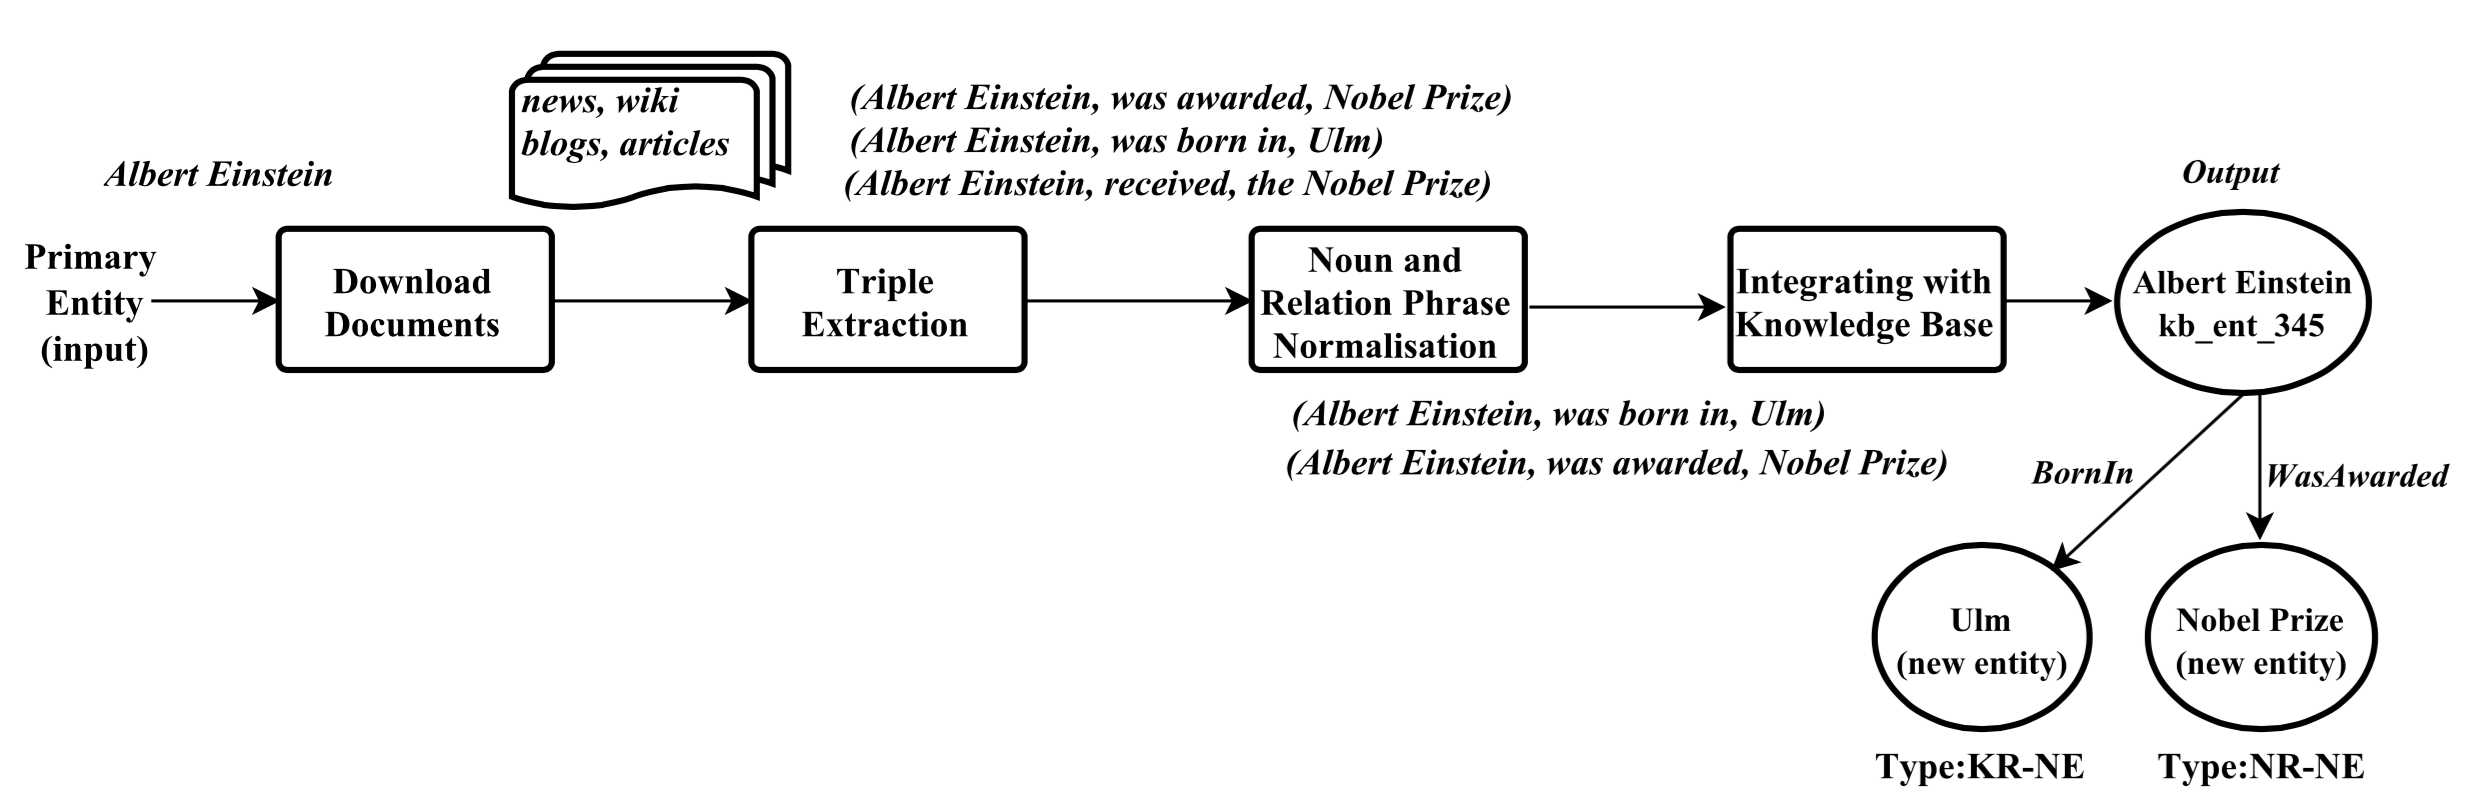
\includegraphics[scale= 0.36]{images/pipeline.png}
\caption{Dataflow and architecture and  of \system{}. See \refsec{sec:method} for details.}
\label{fig:pipeline}
\end{figure*}

Recently, a few \emph{entity-centric} methods have been proposed to increase knowledge density in KGs \cite{gardner2013improving,gardner2014incorporating}. In contrast to the best-effort approaches mentioned above, these entity-centric approaches aim at increasing knowledge density for a \emph{given} entity. A new fact involving the  given entity can belong to one of the four types  shown in \reftbl{tbl:extraction_taxonomy}. Unfortunately, these densifying techniques only aim at identifying instances of known relations among entities already present in the KG, i.e., they fall in the KR-KE type of \reftbl{tbl:extraction_taxonomy}.

In this paper we propose \systemfull{} (\system{}), an entity-centric knowledge densifying framework which, given an entity, is capable of extracting facts belonging to all the four types shown in \reftbl{tbl:extraction_taxonomy}. By using \system{}, we are able to increase NELL's knowledge density by a factor of 7.7\footnote{Measured with respect to the five categories experimented with in the paper. See \refsec{sec:expts} for details.}, while achieving 75.4\% accuracy. %While the framework itself is relatively simple and can be improved,
Our goal here is to draw attention to the effectiveness of entity-centric approaches with bigger scope (i.e., covering all four extraction classes  in \reftbl{tbl:extraction_taxonomy}) towards improving knowledge density, and that even relatively straightforward techniques can go a long way in alleviating low knowledge density in existing state-of-the-art KGs. \system{} code is available at: {\small {\tt https://github.com/malllabiisc/entity-centric- kb-pop}} %\textit{https://github.com/Manjunathhegde/entity-centric-kb-pop}

% They either focus on identifying instances of of known relations among known entities in the KG \cite{gardner2013improving,gardner2014incorporating}, or they require proprietary technologies not available in the public domain \cite{west2014knowledge}.

%While the knowledge density may be computed directly from the number of entities and facts in the KG, we feel it is an important metric which needs to be reported independently. Knowledge densities of a few KGs are shown in 

%A large number of knowledge base (KB) construction projects have recently emerged. Prominent examples include Freebase which powers the Google Knowledge Graph, 
%ConceptNet, YAGO and others. These KBs contain many millions of entities, organized in hundreds to hundred thousands of semantic classes, and hundred millions of relational facts between entities. 
%The approach towards building these knowledge bases is to collect all possible information from the corpus and represent them in the KB. Our approach in constructing entity specific 
%knowledge base is to search for the predefined entities and extract facts related to that. We store the extractions in the form of triples. For the primary entity, extractions will be of the form - (primary entity, relation, entity-2)
%or (entity-2, relation, primary entity)
%Finding the (relation, entity-2) pairs for the given primary entity and classifying them as new or existing information is the aim of this paper. 
%The set of operations are carried out on the subject verb object triples to find the relations and entity-2.
%NELL has the facts related to lot of entities, hence we use it to classify extractions as new or existing fact.
%With the (relation, entity-2) pair gives 5 different combination.\\
%Case 1: both the relation and entity-2 exists in the knowledge base and they are connected. So it is a known fact.
%Case 2: both the relation and entity-2 exists in the knowledge base but they are not connected. So it is a new fact.
%Case 3: relation is present in the KB but entity-2 is new. So system has identified a new entity.
%Case 4: entity-2 is present in the KB but relation is new. So system has identified a new relation.
%Case 5: both entity-2 and relation are new.
%The other sections describe the related work on this topic, methodology in clustering the data and mapping to existing knowledge base.

\section{Related Work}
\label{sec:related}

Open Information Extraction (OIE) systems \cite{textrunner,reverb,ollie} aim at extracting textual triples of the form noun phrase-predicate-noun phrase. While such systems aim for extraction coverage, and because  they operate in an ontology-free setting, they don't directly address the problem of improving knowledge density in ontological KGs such as NELL. 
However, OIE extractions provide a suitable starting point which is exploited by \system{}. \cite{canopy} addresses the problem of normalizing (or canonicalizing) OIE extractions which can be considered as one of the components of \system{} (see \refsec{sec:normalization}). 
\\As a final step of \system{} we map the relation to a nell-relation. There has been many efforts in all three learning paradigms (supervised, semi-supervised and unsupervised) 
for Relation Extraction prior to Distant Supervision. In supervised setting, sentences with labelled entities and relations are used to learn relation extractors in supervised setting.
Work by \cite{zhou122007tree} use supervised datasets to learn classifiers to label the relations mention between a given pair of entities in a test sentence, optionally combining relation mentions.
Supervised learner suffer from problems like expensive labelled data, corpus based relation labels and classifiers tuned for given text corpus.

Other extreme for Relation Extraction is to use completely un-supervised techniques. In this approach, string of words between two entities taken from a large number of unlabelled 
sentences is clustered. Each cluster then signifies a relation-strings. Mapping of relation clusters to knowledge base specific relation is an added overhead in un-supervised approach.
In semi-supervised learning, a very small number of seed instances or patterns are used to do bootstrap learning. \cite{rozenfeld2008self}
Original seed set is used to extract relations patterns, which further generate more instances. New instances are again used to generate relation patterns,
this continues in iterative fashion. This approach suffers from low precision and semantic drift.

As previously mentioned, recent proposals for improving density of KGs such as those reported in \cite{gardner2013improving,gardner2014incorporating} focus on extracting facts of one of the four extraction classes mentioned in \reftbl{tbl:extraction_taxonomy}, viz., KR-KE. The KBP challenge \cite{surdeanu2013overview}  also focuses on extracting facts while keeping the relation set fixed, i.e., it addresses the KR-KE and KR-NE extraction classes.

A method to improve knowledge density in KGs by using search engine query logs and a question answering system is presented in \cite{west2014knowledge}. The proprietary nature of datasets and tools used in this approach limits its applicability in our setting.

\system{} aims to improve knowledge density by extracting facts from all four extraction classes, i.e., for a given entity, it extracts facts involving known relations, identifies potentially new relations that might be relevant for this entity, establishes such relations between the given entity and other known as well as new entities -- all in a single system. While various parts of this problem have been studied in isolation in the past, \system{} is the first system to the best of our knowledge that addresses the complete problem as a single framework.



%To best of our knowledge, no specific paper has discussed populating knowledge bases with entity centric approach. 
%The below subsections discusses the relative works that has been done in information extraction and clustering which are used in our system.
%
%\subsection{Information Extraction}
%\label{sec:inormationextraction}
%Lot of work has been done in creating  knowledge bases and processing the web corpus to represent them in the more  informative way. 
%The \textit{subject verb object} triple extraction problem has been deeply studied and many approaches have been proposed. 
%TextRunner \cite{textrunner} has used Naive Bayer’s classifier and CRF models to identify the noun phrases and the relations in the sentence. 
%Reverb \cite{reverb} approach has followed light verb based model along with the rule based mechanism to define the relation in the sentence and in turn to find the noun phrases. 
%Ollie \cite{ollie} has more general approach to consider noun phrases along with verbs in the relation. 
%OpenIE V4 \cite{openie4} has used the statistical relational learning methods to extract relations.

%\subsection{Clustering Entities and Relations}
%\label{clusterentrel}
%\cite{canopy} summarizes different methods used in clustering the relations and entities. Most of the work in this area mainly talks about defining the similarity between words or phrases.


\begin{table*}[!htb]
\begin{small}
\begin{center}
\begin{tabular}{|p{2cm}|p{2cm}|p{2.5cm}|p{2cm}|p{2cm}|p{2cm}|p{2cm}|}
\hline
%\textbf{Category} & \textbf{Avg.No. of facts/entity in NELL} & \textbf{Avg.No. of facts/entity extracted} & \textbf{Facts Evaluated} & \textbf{No. of Correct Facts} & \textbf{Accuracy}\\
\textbf{Category} & \textbf{Knowledge Density in NELL} & \textbf{Knowledge Density after \system{}} & \textbf{\# Facts Evaluated} & \textbf{\# Correct Facts} & \textbf{Accuracy}\\
\hline
Scientist & 1.27 & 18.5 & 164 & 141 & 85.97 \\
\hline
Universities & 1.17 & 9 & 197 & 141 & 71.57\\
\hline
Books & 1.34 & 4.49 & 202 & 165 & 81.68 \\
\hline
Birds & 1.27 & 6.69 & 194 & 136 & 70.10 \\
\hline
Cars & 1.5 & 11.61 & 201 & 140 & 69.65 \\
\hline
\hline
Overall & 1.3 & 10.05 & 958 & 723 & 75.46 \\
\hline
\end{tabular}
\caption{\label{tbl:main_result}Knowledge densities of five categories in NELL and after application of \system{}, along with resulting accuracy. We observe that overall, \system{} is able to increase knowledge density by a factor of 7.7 at 75.5\% accuracy. This is our main result.}
\end{center}
%\end{table*}
%
%\begin{table*}[th]
%\begin{small}
\begin{tabular}{|p{2.3cm}|p{4.6cm}|p{5.5cm}|p{2cm}|}
%\begin{tabular}{|c|c|c|c|}
\hline
\textbf{Entity Name} & \textbf{All facts in NELL} & \textbf{Sample facts extracted by \system{}} & \textbf{Extraction Class} \\
\hline
%Seth Carlo Chandler & Seth Carlo Chandler can be found on Wikipedia at http://en.wikipedia.org/wiki/ Seth\%20Carlo\%20Chandler & Seth Carlo Chandler became associated with Benjamin Pierce & NR-KE\\ 
%\\
%{} & {} & Chandler used Almucantar & KR-KE \\
%\\
%{} & {} & Seth Carlo Chandler lived on Craigie street & KR-NE \\
%\hline
\textit{George Paget Thomson} & \textit{(George Paget Thomson, isInstanceOf, scientist)} & \textit{(Sir George Thomson, isFellowOf, Royal Society)} & NR-KE \\
%{} & {} & (George Thomson, married, Kathleen Buchanan Smith) & KR-NE \\
{} & {} & \textit{(George Thomson, hasSpouse, Kathleen Buchanan Smith)} & KR-NE \\
{} & {} & \textit{(George Paget Thomson, diedOn,  September 10)} & KR-KE\\
%\hline
%Joseph Engelberger & Joseph Engelberger is a scientist %Joseph Engelberger can be found on Wikipedia at http://en.wikipedia.org/wiki/ Joseph\%20Engelberger 
%	& Joseph Engelberger founded HelpMate Robotics Inc & KR-NE\\
%{} &  & Joseph Engelberger born in New York City & KR-KE\\
%{} & {} & Unimate actually predated Engelberger & NR-NE \\
\hline
\end{tabular}
\caption{\label{table:mapping}Facts corresponding to an entity from the \textit{scientists} domain in NELL as well as those extracted by \system{}. While NELL contained only one fact for this entity, \system{} was able to extract 15 facts for this entity, only 3 of which are shown above.}
%\vspace{0.2cm}
%\end{small}
%\end{table*}
%
%\begin{table*}[th]
%\begin{small}
\begin{tabular}{|p{1.5cm}|p{0.8cm}|p{0.8cm}|p{0.65cm}|p{0.8cm}|p{0.8cm}|p{0.65cm}|p{0.8cm}|p{0.8cm}|p{0.65cm}|p{0.8cm}|p{0.8cm}|p{0.65cm}|}
\hline
\textbf{Category} & \multicolumn{3}{c|}{\textbf{KR - KE}} & \multicolumn{3}{c|}{\textbf{KR - NE}}  & \multicolumn{3}{c|}{\textbf{NR - KE}} & \multicolumn{3}{c|}{\textbf{NR - NE}} \\
\hline
 {} & correct facts & wrong facts  & acc. & correct facts & wrong facts & acc. & correct facts & wrong facts & acc. & correct facts & wrong facts & acc.\\
\hline
Scientists & 57 & 10 & 85.07 & 61& 8 & 88.40 & 14 & 3 & 82.35 & 9 & 2 & 81.81 \\
\hline
Cars & 68 & 35 & 66.01 & 58 & 21 & 73.41 & 9 & 5 & 64.28 & 5 & 0 & 100 \\
\hline
Universities & 52 & 30 & 63.41 & 68 & 20 & 77.27 & 9 & 2 & 81.81 & 12 & 4 & 75 \\
\hline
Books & 78 & 24 & 76.47 & 79 & 12 & 86.81 & 2 & 0 & 100 & 6  & 1  & 85.71 \\
\hline
Birds & 67 & 29 & 69.79 & 46 & 19 & 70.76 & 15 & 4 & 78.94 & 8 & 6 & 57.14 \\
\hline
\hline
Overall & 322	 & 128 & 71.55 & 312 & 80 & 79.59 & 49 & 14 & 77.77 & 40 & 13 & 75.47 \\
\hline
\end{tabular}
\caption{\label{table:precision}Accuracy breakdown over \system{} extractions for each of the four extraction classes in \reftbl{tbl:extraction_taxonomy}. For each category, approximately 200 extractions were evaluated using Mechanical Turk.}
\end{small}
\end{table*}


\section{\systemfull{} (\system{})}
\label{sec:method}

Overall architecture and dataflow within \system{} is shown in \reffig{fig:pipeline}. We describe each of the components in the sections below.

\subsection{Data Preprocessing}
\label{sec:dataextraction}

With Google API, we use RESTful requests to get web search links. Given the primary entity (PE), documents relevant to it are downloaded by issuing queries against Google. In order to make the query specific, especially in case of ambiguous entities, 
a few keywords are also added to the query. For the experiments in this paper, the category is used as the keyword. For example, for the entity \textit{Albert Einstein} from the \textit{scientist}
category, the query will be \textit{"Albert Einstein scientist"}. 
Whenever available, any attribute(s) of the entity is also included as keyword. Since our method is an unsupervised way of expanding the KB, we keep the input from the user to a very minimal extent.   
Entity linking service is used to find the wikipedia page of the primary Entity. This helps us in disambiguating the similar entities and rejecting the wikipedia links of disambiguous entities.
On an avg.top 20 documents returned by the search engine are downloaded and processed further. Number of documents are restricted by the Google API query limits.
Text is extracted from the raw downloaded html documents using regex patters, HTML tag matching, and by using
the Boilerpipe tool\footnote{Boilerpipe: http://code.google.com/p/boilerpipe}.

%The source of data is web documents and searches are made specific to primary entity. Key words related to primary entity are used while querying so as to get more relevant and useful  documents. The key words can be either user specified or domain name to which the entity belongs to. In our work, for most of the experiments domain name was used as the key word. One more approach tried was getting relevant words from knowledge bases. Freebase id of the entity is used to get the attributes from freebase. For e.g. attributes like place and date of birth, religion etc are listed for person category.  These attributes acts as key words and improves the search results.
%Web page contents are downloaded, cleaned and dumped to local system. The processing of the raw data is done using regex pattern matching, HTML tag matching and the Boiler-pipe, a tool to extract text from web documents.

\subsection{Triple Extraction and Processing}
\label{sec:tripleextraction}
Text of each document obtained in the previous step is processed through the Stanford CoreNLP toolkit\cite{manning2014stanford}. Stanford CoreNLP provides a set of natural language analysis tools. It can give the base forms of words, their parts of speech, whether they are names of companies, people, etc., 
normalize dates, times, and numeric quantities, and mark up the structure of sentences in terms of phrases and word dependencies, indicate which noun phrases refer to the same entities. 
We use the sentence tokenization, coreference resolution, NER and POS tags and dependency parsing features of the CoreNLP toolkit.
Sentences without resolving coreference are then passed through OpenIEv4 \footnote{OpenIEv4: http://knowitall.github.io/openie/} to extract  \textit{(noun phrase, predicate,noun phrase)} triples. 
Coref resolution is performed on these triples using the output of CoreNLP toolkit. 
Multiple and overlapping triples from the sentence was permitted. Length filter is applied on the noun phrase and the predicate of the triple extracted. This eliminates
triples whose predicate is more than 6 tokens and noun phrase more than 8 tokens.\\
The above process of representing sentence in a triple form is quite noisy. We loose lot of information when a big sentence is break down to a triple. 
For e.g. A sentence explaining bombing incident may contain place, time, victim, culprit, but OpenIE breaks it into many triples, each of which on their own does not describe the event completely.
Example given below explains the few possibilities of noise induction.\\
Sentence:\textit{In 1940 Albert Einstein renounced his German nationality law for a second time and became a U.S. Citizenship.}\\
OpenIE Extractions:
\begin{itemize}
\item{0.91747 :(Albert Einstein;renounced;his German nationality law)}
\item{0.91747 :(Albert Einstein;renounced;for a second time)}
\item{0.91747 :(Albert Einstein;renounced;In 1940)}
\item{0.95421 :(Albert Einstein;became;a U.S. Citizenship)}
\item{0.95421 :(Albert Einstein;became;In 1940)}
\end{itemize}

Third and the last triple are capturing only time and hence miss the context. Second triple is a not very informative.

\textbf{Entity Disambiguation and Linking:} It is the task of determining the identity of entities mentioned in text.
Named entity mentions can be highly ambiguous, any entity linking method must address this inherent ambiguity, 
We use dexter entity linking system which finds and mapps the entity mentions in the text to wikipedia page titles. 
This phase helps in clustering the different mentions of the same entity.

\textbf{Extraction of Entity from Noun Phrase:}
Even after applying length filter, long noun phrases may not represent a real world entity. Consider the example given below,\\
Sentence:\textit{Soon after their divorce, Albert Einstein married his cousin Elsa.}
\begin{itemize}
\item{0.91746 :(Albert Einstein;married;his cousin Elsa)}
\item{0.91746 :(Albert Einstein;married;Soon after their divorce)}
\end{itemize}
OPenIE extraction has marked \textit{his cousin Elsa} as the Entity-2, but we would like to have \textit{haswife(Albert Einstein,Elsa)} as the instance of the KB. Now the challenge is how to 
select only "Elsa" from "his cousin Elsa". We term this as the task of obtaining entity from noun phrases.
One more challenge here is to filter out the second triple because \textit{haswife(Albert Einstein, divorce)} is an erroneous tuple.\\

To address both the task of obtaining entity from noun phrase and rejecting the wrong triples, we use a scoring mechanism. Scoring mechanism is based on the POS tag patterns of the entities present in wiki dump[ref??]

POS tag patterns of entities from wikipedia dump are mined and stored along with their counts. POS tag of any given noun phrase is matched with the existing POS tag patterns and the best match from phrase is selected as Entity-2.
Frequency of the matched POS tag pattern, ratio of the length of Entity-2 to length of noun phrase and openIE score is used to calculate triple score.\\

Triple Score = Frequency of POS tag * (number of words in Entity-2/Number od words in noun phrase) * OpenIE score\\

%\reminder{MGH: Add example or few top and bottom ranked entities}

% Sentence:\textit{Albert Einstein himself had always opposed long and horrifying war.}\\
% OpenIE Extractions:\\
% \begin{itemize}
% \item{0.92564: (Albert Einstein;had opposed;long and horrifying war)}
% \item{0.92564: (Albert Einstein;had opposed;always)}
% \end{itemize}
% Replace "long and horrifying war" to "war"
% Reject the second triple\\



%Raw data from the web contains many indirect references, so it is also important to address the co-reference resolution problem here. 
%Indirect references can be either pronouns, adjectives or some variations of the entity string. The Stanford co-reference resolution tool is used for sentence tokenizing and coreference resolution. The dependency tree structure is used to extract the entity when the output entity of the Stanford CoreNLP was greater than certain threshold. The sentences formed are used as input to openIE for triple extraction.\\
%OpenIE is a tool to extract triples from the sentences. These output triples have a \textit{subject predicate object} format. 
%The extractions from the OpenIE have the score mentioning the correctness of the extraction. Each sentence will have multiple extractions with different confident scores. 
%We consider multiple extractions from the same sentence. 2 extractions for the sentence \textit{Modi sell tea at vadanagar railway station} were 
%\textit{(Modi, sell, tea)} and \textit{(Modi, sell tea at, Vadanagar railway station)}. Considering both the extractions helps us to find the new entity \textit{vadanagar railway station}.
%Constraints are imposed on the length of the phrases which are acting as relation and entity2. This eliminates the many such phrases which are extracted from OpenIE, 
%but are not representing a real time entity or relation.  

%\subsection{Clustering entities and relations}
\subsection{Noun and Relation Phrase Normalization}
\label{sec:normalization}

Noun phrases (NPs) and relation phrases obtained from the previous step are normalized (or canonicalized) in this step. Canopy clustering technique as proposed in \cite{canopy} was 
used for noun phrase as well relation phrase clustering. 
Initial clustering is done over the \textit{unlinked} noun phrases in the triples. Please note that since we are working in an entity-centric manner, one of the two NPs present in the triple is already connected to the knowledge graph, and hence is considered \textit{linked}. 
To cluster noun phrases, we first construct canopies corresponding to each word in the noun phrase. For example, 
for noun phrase \textit{Albert Einstein}, we create two canopies, viz., a canopy for  \textit{Albert} and another canopy for  \textit{Einstein}, and add \textit{Albert Einstein} to both canopies. 
Grouping of noun phrases inside the canopy is the next step of clustering phase.
Noun phrase similarity is calculated based on  similarity of words in the noun phrases. 
Word similarity is either direct string matching or Gensim similarity score\footnote{https://github.com/piskvorky/gensim/}, which internally uses word2vec
embeddings \cite{mikolov2013distributed}. After calculating pairwise similarity of noun phrases, hierarchical clustering is carried out to group noun phrases inside each canopy. 
A threshold score is used to stop hierarchical clustering. At the end of this process, we have canopies and groups of noun phrases inside them. 
A noun phrase can be in more than one canopy, hence those groups across canopies are merged if the similarity is greater than certain threshold. After this, each group will contain facts which have similar noun phrases and different (or same) relation phrase.
Again the facts are clustered based on the similarity of the relation phrase. Relation phrase similarity calculation step resembles the one used for noun phrases as described above.

After this triple clustering step, the best representative triple from each cluster is selected based on a few rules. We consider the structure of POS tags in noun phrases of a triple as one of the criteria. Secondly, if both noun phrases in the triple are linked to the knowledge graph, then it makes the triple more likely to become a representative tuple of the cluster. Also, if the NPs present in the triple are frequent in the cluster, then it makes the corresponding triple more like to become a representative.

%We consider the structure of POS tags of the noun phrase as one of criteria for selection. %The entities that appear in the document follow some common structure like noun followed by noun or adjective followed by noun. 
%Next criteria is the presence of entity in the triple. The entity2 of the triple if it has a freebase id then it is an evidence that the triple extracted is a useful fact. 
%We also consider the frequency of the noun phrase in the cluster(num of facts having the noun phrase as entity2) for selection.

%The triple extractions from the previous step are clustered in this phase. As the aim is to find (relation, entity) pair for the primary entity from the extractions, grouping is done so that 
%similar extractions lie in a same set. The initial ideas of canopy clustering \cite{canopy} is used for entity and relation cluster. 
%To cluster entities, we first construct canopies. 
%Each word in the entity is either added to a canopy or new canopy is constructed if not present. For entity say \textit{Albert Einstein}, we create 2 canopies namely canopy \textit{Albert} and canopy 
%\textit{Einstein}. Each will have
%the entity \textit{Albert Einstein}. Since the entities inside each canopy share a word, the probability of they being similar is high. Next step is to find the similar entities inside each canopy and group them.
%To find the similarity between two entities we define pair wise similarity function. This function considers each phrase or the entity as the bag of words.
%The string and freebase id matching techniques are used to find the similar entities. When the words don’t match, the gensim model is used to calculate the similarity between the words.
%For e.g., if the entity one has 3 words \textit{w1, w2, w3} and entity two has 2 words \textit{x1, x2}, similarity is calculated as follows, For each word ‘w’ in entity one, find the best
%match in entity 2. If string match of w and x is true, then similarity score is 1, else use the similarity score returned by gensim similarity function. Add all these word wise similarity
%score and divide it by the number of words in the phrase. 
%After the similarity calculation, grouping of entities is done in the following way. Inside every canopy, group those 2 entities which are mutually close to each other into one set. An hierarchical clustering 
%is carried until the similarity is greater than threshold. Merging happens across canopies also. So after the clustering phase, each set will have triples where entities participating are similar. 
%The similarity of relations within each set is calculated for final grouping of the triples. The bag of words and gensim is used again to find relation similarity. After final grouping, each set will have triples which convey the same fact. \\

%\subsection{Entity and Relation Normalization}
%After grouping similar extractions, the best possible candidate from the group is selected based on few rules. 
%The aim of selecting the extraction and cleaning the entity is to represent the extraction as a knowledge fact. This helps us to map the fact to existing knowledge bases. 
%The pos tag structure of entities are studied and the filters (defined in Katz filter) are used to extract the best possible entity structure from the phrase.

%\subsection{Matching extraction to NELL}
\subsection{Integrating with Knowledge Graph OR Relation Mapping}
\label{sec:rel-map}
\subsubsection{ Distance supervision}
\cite{mintz2009distant} proposed distant supervision for the first time in 2009. Their approach uses Freebase, a large semantic database to provide distant supervision for relation extraction. The algorithm
assumes that any sentence containing two entities expresses relation between those two entities as given in freebase.
Unlike supervised setting, this approach is noisy, but can learn well due to large number of examples. 
The algorithm depends on a database for it’s relation instances, and therefore does not suffer from domain-dependence or overfitting.\\
We use distance supervision to map the relation in a triple to a nell-relation. 
The distant supervision assumption is that if two entities participate in a relation, any sentence that contains those two entities might express that relation.
With the above assumption, we generate training data for relation mapping using the instances from NELL. Detailed procedure for generating positive and negative training 
is described below.
Web data is the source of distance supervision for both negative and positive training samples.
For the task of relation mapping, we have hand picked 110 nell-relations.
We are using the high confident nell instances and consider them as the true lables for all of the selected nell-relations.
For each nell-relation we get 100 to 500 instances of the form \{Entity-1:Entity-1-type, Entity-2:Entity-2-type\}


For positive training samples, we take instance pairs (Entity-1,Entity-2) and using the initial part of the pipeline[??], we collect
sentences from web pages. We use wildcard character '*' between entities ("Entity-1 * Entity-2") in the Google search to get more accurate sentences. These sentences contains both entities and hence represent the relation.

Even for negative training samples, we consider same set of nell relations. The generation of instances differs from positive data collection. We take Entity-1 from the instance pair and
Entity-2-Neg is collected as follows, select an entity which has type same as Entity-2 and "Entity-1 nell-relation Entity-2-neg" is not present in NELL.

Example, for nell relation 'personborninlocation', NELL instance pair (Obama:person, Honolulu:location)\\
Sentences selected as positive training example are\\
\begin{itemize}
 \item Barack Hussein Obama, born in Honolulu on August 4, 1961.\\
 \item However, a view of the various homes where Obama dwelled in Honolulu reveals a broader, diversified beginning.\\
\end{itemize}
Examples for negative training.\\
\begin{itemize}
 \item Obama Pokes Fun at Friends and Enemies at dinner held in Washington.\\
 \item Obama walks to stage at rally in Washington.\\
\end{itemize}

There is always a noise factor associated with distance supervision and it affects the accuracy of the system. 

\subsubsection{CNN for Relation Mapping:}
High level architecture of the CNN is shown in \reffig{fig:cnn}
\begin{figure*}[!htbp]
\begin{center}
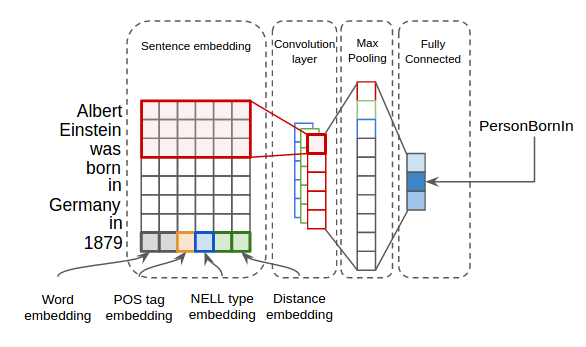
\includegraphics[scale= 1]{images/CNN.png}
\end{center}
\caption{CNN for relation mapping. See \refsec{sec:rel-map} for details.}
\label{fig:cnn}
\end{figure*}
For relation linking, the distantly supervised training data is used to train a classification model. Given an instance, which consists of a plain text sentence, an entity pair, and the NELL type of the entities, the model generates a probability distribution over the candidate relations. 

The classification model used is a Convolutional Neural Network (CNN) following \cite{kim:2014}. In this model, the input instance is represented by an $ n \times d$ \textit{image}, which is then fed through a CNN. Two filters (of height 1 and 2) are used in a single convolution layer, followed by a max-pooling layer. These are 1D (temporal) convolutions, and therefore the width of the filter is equal to the width of the image. The height, therefore, is analogous to the size of a context window around tokens in a sentence.

To convert the raw text into an input image, the following features are used. Each feature is embedded using a matrix of parameters that is learned as part of the training process.

\begin{itemize}
\item Word features: word ids are embedded using an embedding matrix that is initialized using Glove \cite{pennington2014glove} vectors. 
\item POS tags: Generated using CoreNLP
\item NELL type information: Generated using ???
\item Position features: From \cite{zeng:2014}, these features are integers that represent the relative distance of each token from an anchor entity (see Fig.). Two such features are generated, one for each entity in the entity pair. These features are useful in incorporating temporal information about word-ordering into the input, which otherwise a CNN is agnostic to.
\end{itemize}

$d$ is therefore $d_{word} + d_{pos-tag} + d_{NELL-type} + 2\times d_{position})$. $d_{word}$ is set to 300, while all the other embedding matrices are chosen do be 50 dimensional. The number of filters used is 256.

\subsubsection{Relatiom Mapping Using Extraction Patterns}
The set of normalized triples from the previous step are linked with the Knowledge Graph, whenever possible, in this step.
Metadata for each relation in NELL has a set of verb phrases, which capture the variation of the nell-relation in free text.
The similarity of words in triple to avg similarity of words in the extraction pattern is used for relation mapping.
GloVe vector representation of words is the key behind calculating the similarity. GloVe is an unsupervised learning algorithm for obtaining vector representations for words. 
Training is performed on aggregated global word-word co-occurrence statistics from a corpus. Each word is represented as a vector of dimension 300.
The algorithm \ref{alg:RMalgorithm} describes all the steps of relation mapping.
Whenever this extraaction pattern based mapping is not possible, then the predicate is listed as a new relation, and the
corresponding triple marked to belong to either NR-KE or NR-NE extraction class, depending on whether the target entity is already present in the KG or not.

\begin{algorithm}

\caption{Relation Mapping with Extraction Patterns and Glove Vectors}

\label{alg:RMalgorithm}

\begin{algorithmic}[1]

\Procedure{Relation Mapping}{}

\State Triple: \textit{Entity-1,relation,Entity-2}
\State get entity type (\textit{Entity-1-Type,Entity-2-Type}) using NELL Json API

\State relation vector (RV) = initialise 0-vector of length 300
\For{each word in relation}
\State RV = RV + GloVe(word)
\EndFor
\State RV = RV/number of words in relation

\State S = Set(nell-relations which satisy type constraints)
\For{each nell-relation in S}
\State P=Extraction patterns for nell-relation
\For{each extraction-pattern in P}
\State EPV = initialise zero vector
\For{each word in extraction pattern}
\State EPV = EPV + GloVe(word)
\EndFor
\State EPV = EPV/number of words in extraction pattern
\EndFor
\State similarity = cosineSimilarity(RV,EPV)
\EndFor
\State Mapped Relation = relation with maximum similarity score
\EndProcedure
\end{algorithmic}

\end{algorithm}
%%%
%%%
% The set of normalized triples from the previous step are linked with the Knowledge Graph, whenever possible, in this step. For a given normalized triple, 
% following steps are performed as part of linking. First, category of each noun phrase in the triple is obtained based on string matching. In case of no match, refinements like dropping of adjectives, considering only noun phrases are done to for rematching. 
% Now, the relation phrase is mapped to an existing predicate in the KG based on the extraction patterns in the metadata of the target relation (e.g., NELL and many other KGs have such metadata available).
% Candidate predicates are chosen from the above mapped predicates based on category signature of the two noun phrases (i.e. entity1 and entity2). This is possible since the all the predicates in NELL have the type signature defined in the metadata.
% Frequency of the relation phrase in the metadata is used as a criteria to select a candidate from multiple predicates.
% If such category-signature based mapping is not possible, then the predicate is listed as a new relation, and the
% corresponding triple marked to belong to either NR-KE or NE-NE extraction class, depending on whether the target entity is already present in the KG or not.
%%%
%%%

%Problem with openIE kind of fact extractions is that, they can be highly disambiguated. Both entity and relation phrase of the extraction contribute to ambiguity. 
%For e.g. consider a fact Josephine C. Cohen  married  Mollie Levy,  
%The other occurrences of Josephine C Cohen like Cohen, J C Cohen and other relation phrases for married can husband of. 
%These different combination can give rise to different representation for the same fact.
%NELL has metadata for each relation. E.g. \textit{has spouse} is a NELL relation which is mapped to relation phrases like married, husband of, wife of etc. 
%This metadata about the relations is used to map the relation phrase in the extraction to a NELL-relation. It is also important to know the
%types of the entities that are participating with the relation to reduce the ambiguity of the relation mapping. 
%To get the types of the entities and classify the extraction, entities are mapped to NELL Some heuristics are made while matching entities to NELL. 
%Following are the steps followed while matching an entity to NELL. If the exact match of the entity is found then get the type signature of the entity. 
%Remove phrases like Mr. Mrs. Dr. or adjectives from the entity in the extracted fact and then match it to NELL. 

%So for a given fact, following steps are done as a part of mapping. Get the type signature of the entities in the fact. map the relation phrase to NELL-relation 
%based on the type signature of the entities. Mapping a fact to NELL can be either hit or a miss. We call it a hit when both the relation and second entity
%(we know that primary entity is present in NELL ) is present in the knowledge base. Even though both the entity and relation exists in knowledge graph, there may not be an edge connecting those two. 
%So we classify hit into new and existing fact based on the presence of the edge. A miss occurs when either relation or a second entity is absent in the knowledge base. 


\section{Experiments}
\label{sec:expts}

In order to evaluate effectiveness of \system{}, we apply it to increase knowledge density for 100 randomly selected entities from each of the following five NELL categories: \textit{Scientist, Universities, Books, Birds}, and \textit{Cars}. For each category, a random subset of extractions in that category was evaluated using Mechanical Turk. To get a better accuracy of the evaluation, each fact was evaluated by 3 workers. Workers were made to classify each fact as correct, incorrect or can't say. 
Only those facts classified as correct by 2 or more evaluators were considered as correct facts.

{\bf Main Result}: Experimental results comparing knowledge densities in NELL and after application of \system{}, along with the accuracy of extractions, are presented in \reftbl{tbl:main_result}. 
From this, we observe that \system{} is able to improve knowledge density in NELL by a factor of 7.7 while maintaining 75.5\% accuracy.
Sample extraction examples and accuracy per-extraction class are presented in \reftbl{table:mapping} and \reftbl{table:precision}, respectively.

{\bf Noun and Relation Phrase Normalization}: We didn't perform any intrinsic evaluation of the entity and relation normalization step. However, in this section, we provide a few anecdotal examples to give a sense of the output quality from this step. We observe that the canopy clustering algorithm for entity and normalization is able to cluster together facts with somewhat different surface representations. For example, the algorithm came up with the following cluster with two facts: \textit{ \{(J. Willard Milnor, was awarded, 2011 Abel Prize); (John Milnor, received, Abel Prize)\}}. It is encouraging to see that the system is able to put \textit{J. Willard Milnor} and \textit{John Milnor} together, even though they have somewhat different surface forms (only one word overlap). Similarly, the relation phrases \textit{was awarded} and \textit{received} are also considered to be equivalent in the context of these beliefs.
%{\color{blue} It is interesting to see the type of clusters formed and reason for those cluster formation. The detailed evaluation of the clustering and normalization stage were not done, but the overall quality of the cluster formation and performance of the system was found to be satisfactory.
%For example in the below cluster, \\
%\textit{ \{(J. Willard Milnor, was awarded, 2011 Abel Prize); (John Milnor, received, Abel Prize)\}}\\
%The system has able to cluster facts which have different wordings in relation and entity phrases. In entity matching step, cases where one noun phrase is a substring of other, as in \textit{Abel Prize} and \textit{2011 Abel Prize} are put together.
%This works well in most of the cases but formation of clusters like \textit{1.\{(Indian), (Indian Institute of Science)\}} or \textit{2. \{(America and China),(America)\}} may not be a correct ones.
%
%Consider the example below, \\
%\textit{(Georg Waldemar Cantor, died on, January 6) \\
%(Georg Cantor,died on, January 1918)\\
%}
%These similar facts were placed in different clusters as the number part of the noun phrases are not matching. The canopy method with word level similarity matching may not be suitable for numbers and dates.
%} 

{\bf Integrating with Knowledge Graph}: Based on evaluation over a random-sampling, we find that entity linking in \system{} is 92\% accurate, while relation linking is about 70\% accurate.

In the entity linking stage, adjectives present in a noun phrase (NP) were ignored while matching the noun phrase to entities in the knowledge graph (NELL KB in this case). In case the whole NP didn't find any match, part of the NP was used to retrieve its category, if any. For example, in \textit{(Georg Waldemar Cantor, was born in, 1854)}, the NP  \textit{Georg Waldemar Cantor} was mapped to category \textit{person} using his last name and \textit{1854} to category \textit{date}. The relation phrase \textit{"was born in"} maps to many predicates in NELL relational metadata. NELL predicate \textit{AtDate} was selected based on the rule that category signature of the predicate matches the category of the noun phrases present in the triple. It also has the highest frequency count for the relational phrase in the metadata.

We observed that relation mapping has lesser accuracy due to two reasons. Firstly, error in determining right categories of NPs present in a triple; and secondly, due to higher ambiguity involving relation phrases in general, i.e., a single relation phrase usually matches many relation predicates in the ontology.

%{\color{blue}  In entity linking stage, titles and adjective of the noun phrases were removed while matching it to NELL. Part of the noun phrases were used to get the type in the cases were whole noun phase has no mention in NELL.
%In the following example, \\
%\textit{(Georg Waldemar Cantor, was born in (AtDate), 1854)\\}
%noun phrase \textit{Georg Waldemar Cantor} was mapped to category \textit{person} using his last name and \textit{1854} to category \textit{date}. The relation phrase \textit{was born in} maps to many predicates in NELL relational metadata.
%Predicate \textbf{AtDate} was selected based on the rule that type signature of the predicate matches the type of the noun phrases present in the fact. It also has the highest frequency count for the relational phrase in the metadata.
%In the example below,\\
%\textit{(Christiaan Eijkman, married (SpecializationOf), Aaltje Wigeri Edema)}\\
%\textit{married} has been mapped to \textit{SpecializationOf} because of error in finding the type for \textit{Aaltje Wigeri Edema}
%Relation mapping has lesser accuracy due to 2 reasons. 1. Error in getting type (category) of an entity and 2. Error in selecting a predicate when relation phrase matches many predicates in the metadata.
%}


%For our experiments, NELL knowledge base is chosen for comparison and mapping. Entities for the experiments are selected from NELL. 5 categories are chosen so as to test the working of 
%the system on different  kinds of entities. Subset of nearly 100 entities are randomly selected from NELL's collection. 
%The set of operations discussed in the previous section are performed on the selected entities. The number of queries made to get the entity related links was limited by query quota. Less than 20 documents per entity were selected for further processing. Few examples of the fact extracted are given in the table.  

%Only those extractions having the mention of primary entity are retained in the final result set. These extractions are evaluated through mechanical turk and majority of the answer is considered to assign label. These facts are again evaluated to ensure that labels are correct. 
%The  results from the evaluation and summary of all the facts for different categories are given in the table \ref{table:precision}.

%One more important outcome of these experiments was the category specific relations. After looking at all the extractions of a particular category, we were able to extract relational phrases which were
%highly related to category under observation. Only those phrases which occurs with high frequency were selected and tabulated below. Due to space constraints only few relations for only 2 categories are shown

%The mapping of the extraction to an existing knowledge base was a way to classify the extractions. The classification of the facts were done based on the novelty of the relation and entity as
%discussed in the introduction section. 
%Table \ref{table:mapping} gives few sample outputs of facts that were mapped to NELL. 


%The initial goal of this work was to reduce the sparsity of the knowledge bases by actively populating the facts at entity level. The extractions are classified based on their novelty and correctness of the 
%facts in each class is studied. It is also important to maintain the quality of the facts while expanding the knowledge graph. In our work we see that on an average the increase in the facts are x times 
%with a y \% precision. Table \ref{table:precision} summarizes precision and recall of the facts extracted.
%
%
%
%Table \ref{table:recall} summarizes the average number of facts per entity before and after running our extractor system.



\section{Conclusion}
\label{sec:conclusion}

This paper presents \system{}, a simple but effective entity-centric framework for increasing knowledge densities in automatically constructed knowledge graphs. We find that \system{} is able to significantly increase NELL's knowledge density by a factor of 7.7 at 75.5\% accuracy. In addition to extracting new facts, \system{} is also able to extend the ontology. Our goal in this paper is twofold: (1) to draw attention to the effectiveness of entity-centric approaches with bigger scope (i.e., covering all four extraction classes in Table 1) towards improving knowledge density; and (2) to demonstrate that even relatively straightforward techniques can go a long way in alleviating low knowledge density in existing state-of- the-art KGs. 
Future work will include noise reduction in the pipeline. Close examining of sentences while constructing triples to make sure that noisy triples are not added to the system.

\system{} can be applied to other knowledge graphs with appropriate changes. Experiment with other normalization and relation mapping algorithms are the part of future work.
%we hope to experiment with more sophisticated algorithms as \system{}  components (e.g., normalization and linking modules) in hope of even better performance.

%This paper gives a simple but effective way of solving spareness of the knowledge bases.
%The quality of the extraction depends on the occurrence of the entity name in the web documents. Extractions for categories like Scientists, Universities and car manufacturers were better compared to books because
%of the same reason. 
\section*{Acknowledgment}
I would like to thank Dr. Partha Talukdar for his valuable guidance and support throught the project.
Special thanks to Tushar Nagarajan for building the CNN model and helping me throught the relation mapping process.
All the other members of the Machine and Language Learning (MALL) lab friends for their suggestions and timely help.
I thank MALL lab and Computational and Data Science Department for providing Computational facilities.

\bibliographystyle{IEEEtran}
\bibliography{template}

\end{document}

